% Source of the figure clause-thread.pdf (the clause thread of a clause with the literal signs +, -, +).
% Compile with pdfLaTeX; the PDF is included in the manuscript at its natural size.
\documentclass[tikz,border=1pt]{standalone}
\usepackage[T1]{fontenc}
\usepackage{stix}
\pdfinfoomitdate=1 \pdftrailerid{} \pdfsuppressptexinfo=-1
\definecolor{threadred}{RGB}{200,40,40}
\begin{document}
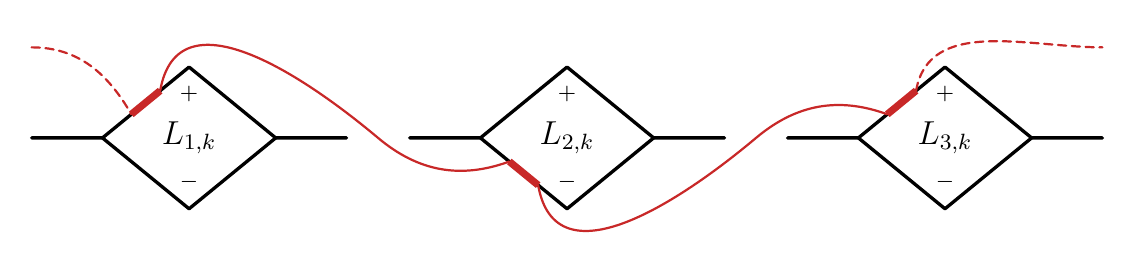
\begin{tikzpicture}[x=1cm, y=1cm,
    chain/.style={line width=1.2pt, line cap=round, line join=round},
    thread/.style={line width=0.8pt, line cap=round},
    crossing/.style={line width=2.6pt, line cap=butt},
    lead/.style={thread, densely dashed}]
  % A chain link with the two single edges next to it: #1 = x-coordinate of its center, #2 = its name.
  % The upper path is the positive path, the lower path the negative path.
  \newcommand{\chainlink}[2]{%
    \draw[chain] (#1-2.0,0) -- (#1-1.1,0) -- (#1,0.9) -- (#1+1.1,0) -- (#1+2.0,0);
    \draw[chain] (#1-1.1,0) -- (#1,-0.9) -- (#1+1.1,0);
    \node at (#1,0) {\large #2};
    \node at (#1,0.56) {\footnotesize $+$};
    \node at (#1,-0.56) {\footnotesize $-$};}
  % A thread at one chain link: #1 = color, #2 = x-coordinate of the center of the link, #3 = 1 (positive
  % path) or -1 (negative path). Draws the crossing edge on the left half of the chosen path.
  \newcommand{\crossingedge}[3]{%
    \draw[crossing, #1] (#2-0.733,#3*0.3) -- (#2-0.367,#3*0.6);}

  \useasboundingbox (0.15,-1.4) rectangle (13.85,1.4);
  \chainlink{2.2}{$L_{1,k}$}
  \chainlink{7.0}{$L_{2,k}$}
  \chainlink{11.8}{$L_{3,k}$}

  % clause thread: positive in L_{1,k}, negative in L_{2,k}, positive in L_{3,k}
  \draw[lead, threadred] (0.2,1.15) to[out=0, in=120] (1.467,0.3);
  \draw[thread, threadred] (1.833,0.6) to[out=80, in=140, looseness=1.15] (4.6,0)
                                       to[out=-40, in=-160] (6.267,-0.3);
  \draw[thread, threadred] (6.633,-0.6) to[out=-80, in=-140, looseness=1.15] (9.4,0)
                                        to[out=40, in=160] (11.067,0.3);
  \draw[lead, threadred] (11.433,0.6) to[out=80, in=180] (13.8,1.15);
  \crossingedge{threadred}{2.2}{1}
  \crossingedge{threadred}{7.0}{-1}
  \crossingedge{threadred}{11.8}{1}
\end{tikzpicture}
\end{document}
